\section{V8}
\subsection{Stack Push und Pop}
\begin{multicols}{2}
 \begin{minipage}{3cm}
     PUSH \qquad {R0}\newline
     PUSH \qquad {R1}\newline
     PUSH \qquad {R2}\newline
     POP \qquad {R3}\newline
     POP \qquad {R4}\newline
     POP \qquad {R5}\newline
 \end{minipage}
 \begin{minipage}{\linewidth}
    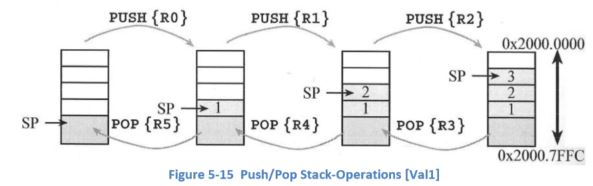
\includegraphics[width=1.5\linewidth]{images/stackpushpop}  
        \end{minipage}
\end{multicols}

\subsubsection{Generelle Regeln bei der Verwendung des Stacks}
\begin{multicols}{2}
\begin{enumerate}
    \item Funktionen sollten die gleiche Anzahl Push und Pop Befehle aufweusen
    \item Stackzugriffnur inerhalb des allozierten Bereichs
    \item Es sollte nicht über den SP auf den Stack geschrieben oder gelesen werden
    \item Stack sollte zuerst den SP dekrementieren und erst dann die Daten ablegen
    \item Stack sollte die Daten zuerst lesen und erst dann den SP inkrementieren
\end{enumerate}
    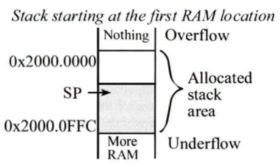
\includegraphics[width=0.8\linewidth]{images/allocatedStack}  
\end{multicols}
\subsection{Shift and Rotate}
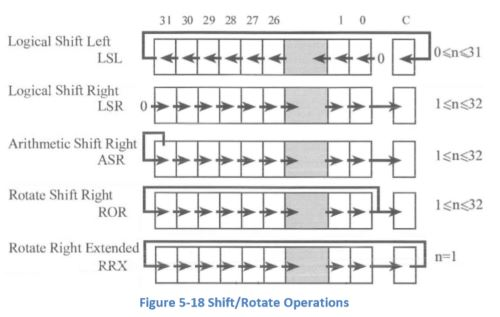
\includegraphics[width=0.8\linewidth]{images/shiftandrotate} 